% Safety by typing: well-formedness + projection implies the three safety properties,
% each discharged by a named Rocq result. Palette: hypothesis=indigo, conclusion=green,
% proof=slate.
\documentclass[border=10pt]{standalone}
\usepackage{tikz}
\usepackage{amsmath}
\usepackage{amssymb}
\usepackage{xcolor}
\usetikzlibrary{arrows.meta, positioning}
\definecolor{hyp}{HTML}{3730A3}
\definecolor{good}{HTML}{16A34A}
\definecolor{proof}{HTML}{475569}
\begin{document}
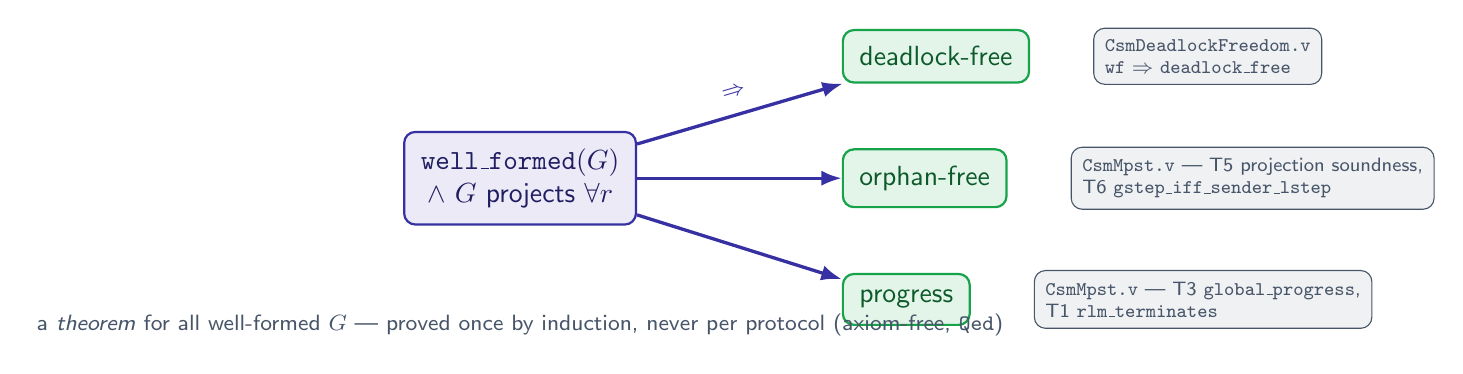
\begin{tikzpicture}[font=\sffamily, >={Latex[length=2.6mm]}, node distance=8mm,
    hyp/.style={draw=hyp, thick, rounded corners, fill=hyp!10, align=center, inner sep=6pt, text=hyp!60!black},
    good/.style={draw=good, thick, rounded corners, fill=good!12, align=center, inner sep=6pt, text=good!55!black},
    pf/.style={draw=proof, thin, rounded corners, fill=proof!8, align=left, inner sep=4pt, font=\sffamily\scriptsize, text=proof}]

  \node[hyp] (wf) {$\mathtt{well\_formed}(G)$\\$\wedge\ G \text{ projects } \forall r$};
  \node[good, above right=6mm and 26mm of wf] (df) {deadlock-free};
  \node[good, right=26mm of wf] (of) {orphan-free};
  \node[good, below right=6mm and 26mm of wf] (pr) {progress};

  \draw[->, hyp, very thick] (wf) -- node[above, sloped, font=\sffamily\footnotesize\bfseries, text=hyp]{$\Rightarrow$} (df);
  \draw[->, hyp, very thick] (wf) -- (of);
  \draw[->, hyp, very thick] (wf) -- (pr);

  \node[pf, right=8mm of df] {\texttt{CsmDeadlockFreedom.v}\\$\mathtt{wf} \Rightarrow \mathtt{deadlock\_free}$};
  \node[pf, right=8mm of of] {\texttt{CsmMpst.v} — T5 projection soundness,\\T6 \texttt{gstep\_iff\_sender\_lstep}};
  \node[pf, right=8mm of pr] {\texttt{CsmMpst.v} — T3 \texttt{global\_progress},\\T1 \texttt{rlm\_terminates}};

  \node[font=\sffamily\footnotesize, text=proof, below=10mm of wf, align=center]
    {a \emph{theorem} for all well-formed $G$ — proved once by induction, never per protocol (axiom-free, \texttt{Qed})};
\end{tikzpicture}
\end{document}
